\documentclass[11pt,ngerman]{scrartcl}

% standard packages
\usepackage[utf8]{inputenc}  % input in UTF-8
\usepackage[T1]{fontenc}  % output in T1 fonts (westeuropäische Codierung)
\usepackage{lmodern}  % latin modern fonts
\usepackage[ngerman]{babel}  % deutsches Sprachpaket, neue Rechtschreibung

% Seitensetup
\usepackage{scrlayer-scrpage}  % Seitenformatierung durch KOMA-interne Optionen
\usepackage[top=4cm, bottom=4cm]{geometry}  % Seitengeometrie (kann durch KOMA ersetzt werden, hab ich aber nicht geschafft)
\usepackage[hypcap=false]{caption, subcaption}  % caption editing - hypcap warning with hyperref
\usepackage{array}  % table editing

% additional packages
\usepackage{amsmath, amssymb, amstext}  % math packages (American Math Society)
\usepackage{bm}
\usepackage{icomma}  % Kommata in Dezimalzahlen verursachen keinen Abstand mehr
\usepackage{graphicx}  % Bilder einfügen
\usepackage{float} %Bilder placement
\usepackage{pdfpages}  % PDF als vollständige Seiten einfügen
\usepackage{lastpage}  % referenziert die letzte Seite
\usepackage[separate-uncertainty=true]{siunitx}  % bessere Darstellung von Einheiten
\usepackage{makecell} %Dicke Tabellenstriche
\usepackage{longtable}
\usepackage{booktabs}
%\usepackage{datatool}
\usepackage[hidelinks]{hyperref}  % hyperref verlinkt Referenzen - hidelinks entfernt borders um links

% package setups
% Kopf- und Fußzeile durch KOMA
\pagestyle{scrheadings}  % KOMA darf entscheiden
\clearpairofpagestyles  % reset
\setkomafont{pageheadfoot}{\normalfont}  % Standardschrift in Kopf- und Fußzeile
\captionsetup{format=plain, font=small, labelfont=bf} %Better caption, Abbildung ist FETT
%\setlength{\headheight}{27.2pt}  % benötigte Höhe Kopfzeile (warning von scrlayer-scrpage, wird aber automatisch so gerendert, falls diese Option weggelassen wird)
\ihead{Halbschattenpolarimeter}  % Kopf links %Todo Titel ändern
\chead{\textsc{Philipp} Maximilian \\ \textsc{Stark} Matthias}  % Kopf Mitte %Todo Name ändern
\ohead{19 November 2021}  % Kopf rechts %Todo Datum ändern
\cfoot{\pagemark \, / \pageref{LastPage}}  % Fuß Mitte

% Table of Contents
\DeclareTOCStyleEntry{dottedtocline}{section}  % KOMA intern - Inhaltsverzeichnis mit Punkten (nur sections)

%Overbar setup
\newcommand{\overbar}[1]{\mkern 1.5mu\overline{\mkern-1.5mu#1\mkern-1.5mu}\mkern 1.5mu}
% SI
\sisetup{locale = DE}  % deutschsprachige SI-Konvention
\sisetup{quotient-mode = fraction}
\sisetup{per-mode = fraction}
\DeclareSIUnit\px{px}
\DeclareSIUnit\strich{|||}

% citation
\usepackage{csquotes}
%\usepackage[backend=biber]{biblatex}

\usepackage[backend=biber]{biblatex}
\addbibresource{halbschatten.bib} %Todo .bib befüllen zb.: mit JabRef (Empfehlung der Redaktion)

%Eigene Commands
\newcommand{\der}[2]{\frac{\mathrm{d}#1}{\mathrm{d}#2}}
\newcommand{\pder}[2]{\frac{\partial #1}{\partial #2}}

%\noindent für ges
\setlength{\parindent}{0pt}


\begin{document}
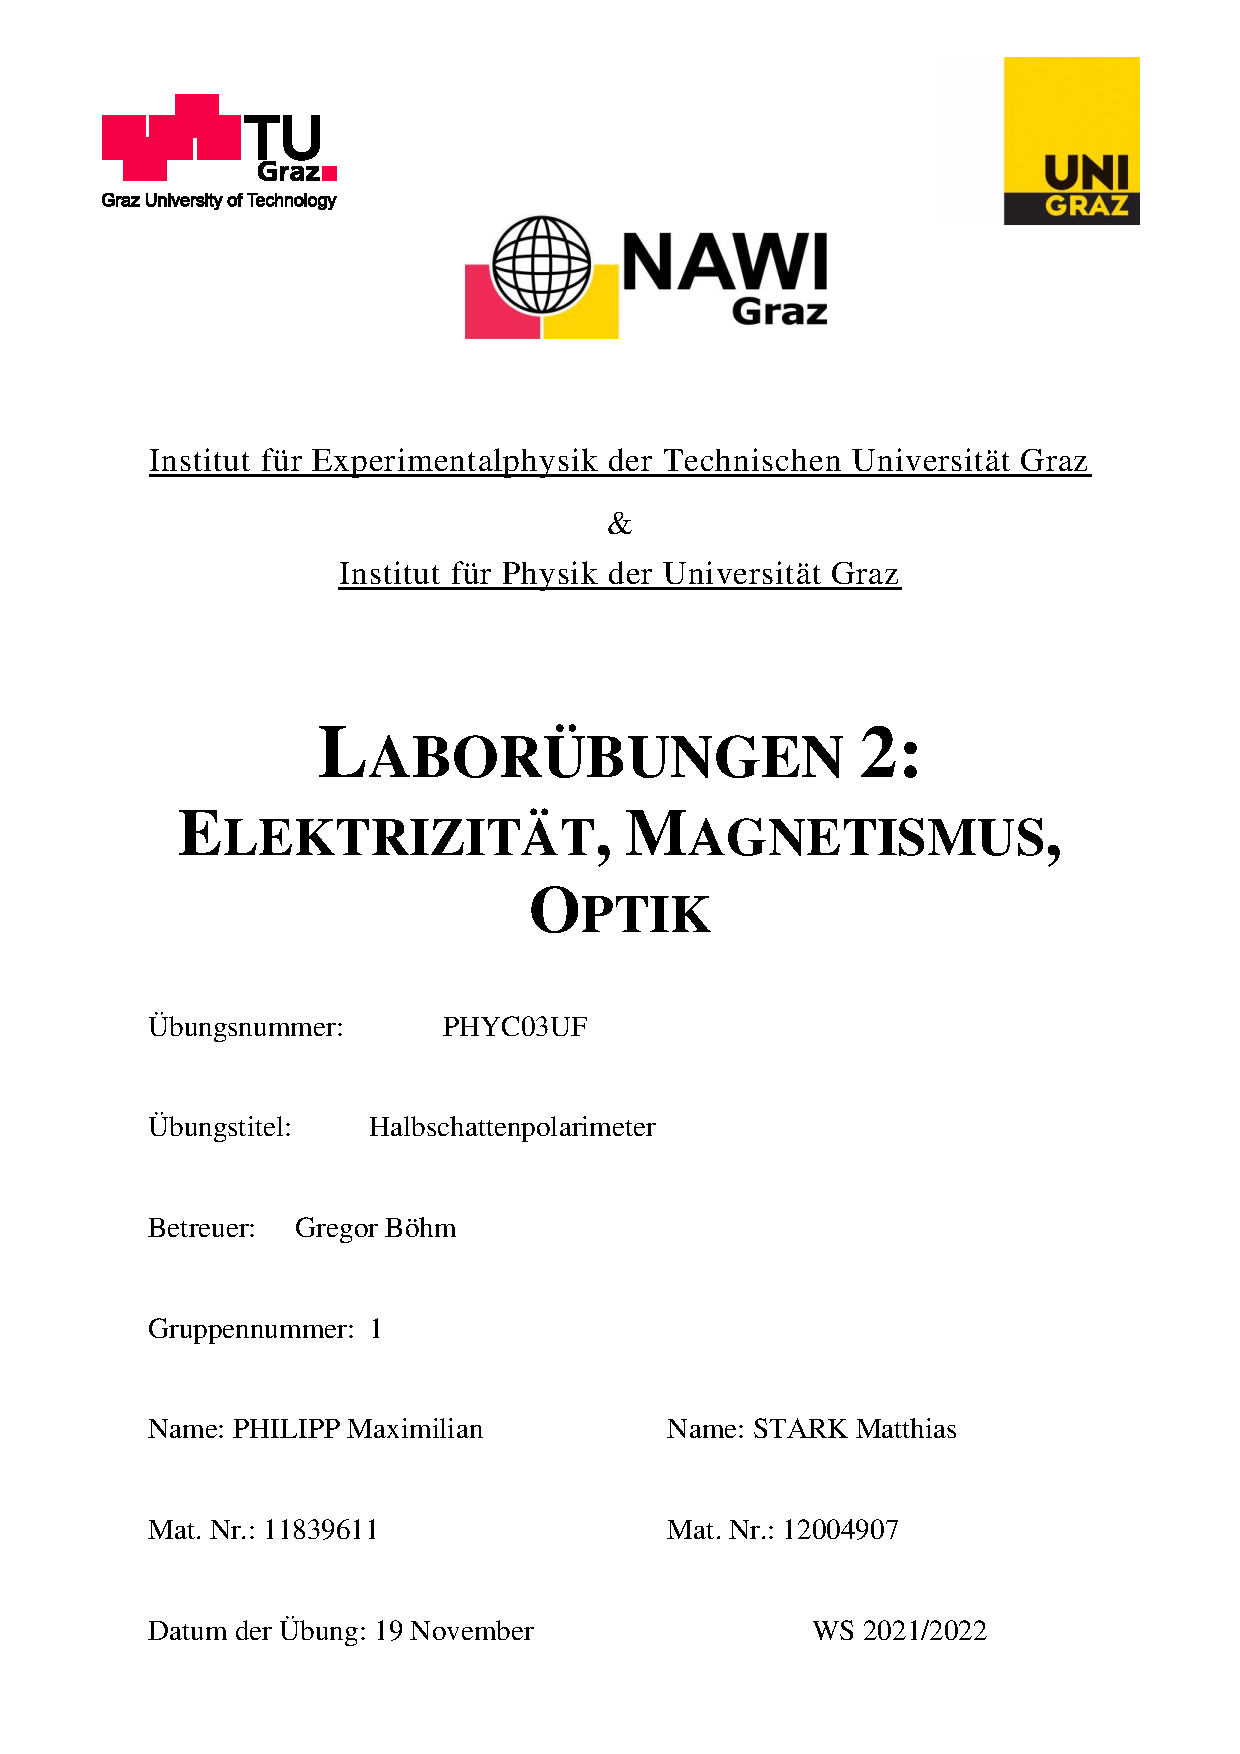
\includepdf{Deckblatt_labor2.pdf}
\tableofcontents
\newpage

\section{Aufgabenstellung\label{Auf0}}

\begin{itemize}
	\item Bestimmung der Konzentration einer Rohrzuckerlösung

	\item Bestimmung der spezifischen Drehung einer Quarzplatte
\end{itemize}


\section{Grundlagen}

Optisch aktiv sind solche Substanzen, die die Schwingungsebene linear polarisierten Lichts nach
rechts oder links drehen. Die Drehrichtung ist vom Beobachter her definiert (Drehung im Uhrzeigersinn
= rechtsdrehend). Es gibt feste, flüssige, aber auch gasförmige optisch aktive Substanzen.
Die wichtigste feste ist der Quarzkristall.

Quarz kristallisiert in zwei spiegelsymmetrischen Formen, Rechts- und Linksquarz. Quarzschmelze (Raumgitter ist zerstört) besitzt keine optische
Aktivität. Das ist ein Beweis, dass bei Quarz und allen sich analog verhaltenden Kristallen
die Gitterstruktur die Ursache der Drehung ist. Die Kristallographie nennt zwei spiegelbildliche
Kristalle ``enantiomorph``. Die Siliziumatome im Quarz sind schraubenförmig angeordnet. Man
kann durch schraubenförmige Anordnung von nicht drehenden Kristallplättchen eine Drehung
der Lichtschwingungsebene erreichen.

Außer den Kristallen drehen auch viele Flüssigkeiten und Lösungen die Schwingungsebene.
Rechtsdrehend sind z.B. Rohrzuckerlösungen, sowie Lösungen von Traubenzucker. Nach links
drehen Nikotin, Chinin usw. Die Drehung der Schwingungsebene durch flüssige oder gasförmige
Stoffe hat ihre Ursache im Bau der jeweiligen Moleküle selbst.

In organischen Stoßen sind einige Kohlenstoffatome asymmetrisch angeordnet, und zwar so,
dass ein C-Atom mit vier ungleichen Atomen oder Atomgruppen verbunden ist. Ein organischer
Stoff, der rechts- oder linksdrehend ist, hat zwar in beiden Fällen dieselbe chemische Formel, die
räumliche Anordnung der Atome bzw. Atomgruppen in beiden Modifikationen lassen sich durch
Translationen kombiniert mit Rotationen nicht zur Deckung bringen (sondern eben nur durch
Spiegelungen).

Die klassische Vorstellung der Drehung der Schwingungsebene ist folgende: Jede lineare Schwingung
kann man sich aus zwei entgegengesetzt zirkularen Schwingungen halber Amplitude aber
gleicher Frequenz zusammengesetzt denken (Fresnel).

Man kann daher auch jede linear polarisierte Lichtquelle in zwei zirkular polarisierte zerlegen.
Nimmt man nun an, dass bei Fortpflanzung parallel der Achse einer aktiven Substanz diese
zirkularen Wellen Realität besitzen, und sich mit verschiedener Geschwindigkeit ausbreiten, so
setzen sich die beiden Anteile beim Austritt aus der Substanz wieder zu einer linear polarisierten
Welle zusammen, deren Schwingungsebene aber gegenüber der einfallenden um einen
bestimmten Winkel gedreht ist. Dieser fällt bei gleicher Wegstrecke umso größer aus, je größer
die Differenz der Geschwindigkeiten ist. Dieser Effekt ist frequenzabhängig, es existiert eine
Rotationsdispersion.

\newpage

Für optisch aktive Lösungen gilt folgender Zusammenhang:

\begin{equation}
	\alpha = (\alpha)Lc
	\label{eq:konz}
\end{equation}

$\alpha$ beschreibt dabei den verursachten Drehwinkel, ($\alpha$) den spezifischen Drehwinkel des Stoffs, $L$ die Länge der durchlaufenden Probe und $c$ die gesuchte Konzentration der Lösung.

\vspace{2mm}

Für die Bestimmung der optischen Aktivität der Quarzplatten wird folgende Formel verwendet, wobei $d$ die Dicke der entsprechenden Probe beschreibt.

\begin{equation}
	\alpha = (\alpha)d
	\label{eq:quarz}
\end{equation}


\section{Versuchsanordnung}\label{sec:Versuchsanordnung}

Die Versuchsanordnung ist in folgender schematischen Skizze ersichtlich:

\begin{figure}[H]
	\begin{center}
		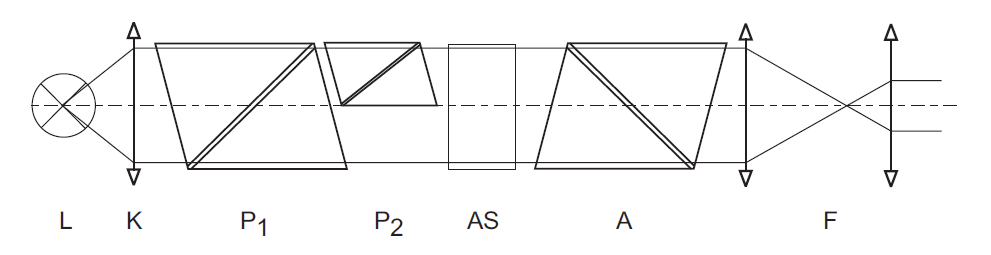
\includegraphics[width=\textwidth]{abb1}
	\end{center}
	\caption{Aufbau des Halbschattenpolarimeters}
	\label{fig:abb1}
\end{figure}

Durch einen Kondensor K wird Licht aus einer Na-Dampflampe L parallel gemacht. Durch
den Polarisator $P_1$ wird linear polarisiertes Licht ($\lambda$ = 5890 $\mathring{A}$ und 5896 $\mathring{A}$) erzeugt, und dessen
Schwingungsebene anschließend in der optisch aktiven Substanz AS gedreht. Mit Hilfe des
Analysators A und des Fernrohres F wird diese Drehung gemessen. Der kleine Polarisator $P_2$
bedeckt den halben Strahlengang, und ist gegen die Schwingungsebene des Polarisators um einen
kleinen Winkel $\alpha \approx $4° gedreht. Ohne dieses sogenannte Halbschattenprisma müsste man den
Analysator auf maximale Helligkeit bzw. Dunkelheit einstellen. Dafür ist das Auge aber nicht so
empfindlich, wie wenn man auf gleiche Helligkeit (geringe) zweier Flächen einstellt. Bei Quarz
ist es wichtig, dass die Drehung der Schwingungsebene nur parallel zur optischen Kristallachse
stattfindet. Schon eine kleine Abweichung bringt sie zum Verschwinden. Die Drehung ist wellenlängenabhängig, für kleines $\lambda$ ist die Drehung größer als für großes. Die Drehung ist also nur
für eine bestimmte Wellenlänge anzugeben, daher monochromatisches Licht. Dieses ist meist die
Fraunhofer'sche D-Linie $\bar{\lambda}$ = 5893 $\mathring{A}$.

Die Trennungslinie der Gesichtsfeldhälften ist die dem Auge zugewandte scharf angeschliffene
Kante des Halbschattenprismas.


\section{Geräteliste}

\noindent Für die Messungen wurden folgende Geräte verwendet:

\captionof{table}{Verwendete Geräte }
\begin{center}
	\begin{tabular}{|c|c|c|c|} \hline
		\textbf{Gerät}             & \textbf{Typ}       & \textbf{Hersteller} \\ \hline

		NA- Dampflampe             & G 22               &                     \\ \hline
		Trafo                      & V / 667 / 2        & Philips             \\ \hline
		Halbschattenpolarimeter    & 2658               & G: Steeg \& Reuter  \\ \hline
		Röhre mit Rohrzuckerlösung & 200 mm             &                     \\ \hline
		Quarzkristall              & 1                  &                     \\ \hline
		Quarzkristall              & 2                  &                     \\ \hline
		Quarzkristall              & 3                  &                     \\ \hline
		Quarzkristall              & 4                  &                     \\ \hline
		Mykrometerschraube         & 102-217 / 0J051184 & Mitutoya            \\ \hline
	\end{tabular}
\end{center}

\section{Versuchsdurchführung \& Messergebnisse}\label{sec:Versuchsdurchführung}

Bei den Messungen ist darauf zu achten, dass die Lampe schon einige Zeit laufen muss, um sicherzustellen, dass ein konstantes Spektrum ausgestrahlt wird.

Zunächst muss, als Referenzwert, der Winkel des Analysators bestimmt werden, bei dem beide Hälften des fokussierten Kreises in der gleichen Intensität erscheinen. Dies ist, aufgrund der Anordnung, an zwei Punkten möglich. Weil der dunkler erscheinende, also der an dem die Vektoren des Lichts antiparallel aufeinander stehen, mit dem menschlichen Auge leichter feststellbar ist, wird dieser für die weitere Auswertung herangezogen.

Um die Kante zwischen den beiden Bereichen besser klar ersichtlich zu machen, muss diese durch Bewegen der Linse scharf gestellt werden. Der entsprechende Winkel kann nun mithilfe der eingebauten Lupe anhand des Nonius abgelesen werden.

\vspace{2mm}

Die Messung des Referenzwinkels $\varphi_0$ wird mehrmals durchgeführt, was folgende Werte liefert:

\begin{table}[H]
	\caption{Messung des Referenzwinkels \\ $\varphi_0 \dots$ gemessener
		Referenzwinkel \\ $\Delta\varphi_0 \dots$ entsprechende Unsicherheit des
		Referenzwinkels}
	\label{tab:refwinkel}
	\centering
	\begin{tabular}{lrr}
\toprule
{} &  $\varphi_0$ / \si{\degree} &  $\Delta \varphi_0$ / \si{\degree} \\
\midrule
0 &                        15.0 &                               0.15 \\
1 &                        14.9 &                               0.15 \\
2 &                        15.0 &                               0.15 \\
3 &                        14.9 &                               0.15 \\
4 &                        15.3 &                               0.15 \\
5 &                        15.2 &                               0.15 \\
6 &                        15.3 &                               0.15 \\
\bottomrule
\end{tabular}

\end{table}

\subsection{Konzentration der Rohrzuckerlösung}

Um die Konzentration der Rohrzuckerlösung zu bestimmen, muss zunächst die Länge $L$ der Probe in Erfahrung gebracht werden. Diese ist im konkreten Fall mit einem Wert von

\begin{align*}
	L = \SI{200.0(5)}{\mm}
	\label{eq:langewert}
\end{align*}

gegeben.

\vspace{2mm}

Nun wird die Probe in die Vorrichtung gegeben und diese wieder geschlossen, um kein Licht von außen zuzulassen.

Durch Verdrehung des Analysators wird nun wieder, wie bereits oben für den Referenzwinkel erwähnt, der Winkel bei der Rohrzuckelösung bestimmt, was folgende Werte liefert:

\begin{table}[H]
	\caption{Messung des Winkels mit der Rohrzuckerlösung \\ $\alpha_L \dots$
		gemessener Winkel \\ $\Delta\alpha_L \dots$ entsprechende Unsicherheit des
		Winkels}
	\label{tab:loswinkel}
	\centering
	\begin{tabular}{lrr}
\toprule
{} &  $\alpha_{L}$ / \si{\degree} &  $\Delta \alpha_{L}$ / \si{\degree} \\
\midrule
0 &                         39.2 &                                0.15 \\
1 &                         39.3 &                                0.15 \\
2 &                         39.0 &                                0.15 \\
3 &                         39.2 &                                0.15 \\
4 &                         39.3 &                                0.15 \\
5 &                         39.1 &                                0.15 \\
6 &                         39.0 &                                0.15 \\
7 &                         39.0 &                                0.15 \\
8 &                         39.1 &                                0.15 \\
9 &                         39.4 &                                0.15 \\
\bottomrule
\end{tabular}

\end{table}

\newpage

\subsection{spezifische Drehung von Quarzplatten}

Zunächst müssen die Dicken der Quarzkristalle bestimmt werden. Dazu werden deren Dicken mit einer Mikrometerschraube gemessen. Um leichte Unebenheiten an der Oberfläche der Platten festzustellen, werden diese an 10 verschiedenen Punkten vermessen, was in folgender \autoref{tab:dicken} angeführt ist.

\begin{table}[H]
	\caption{Messwerte der Dicken der Quarzkristalle \\ $d_{Q_1} \dots$ gemessene
		Dicke für Quarzkristall 1 \\ $d_{Q_2} \dots$ gemessene Dicke für
		Quarzkristall 2\\ $d_{Q_3} \dots$ gemessene Dicke für Quarzkristall 3\\
		$d_{Q_4} \dots$ gemessene Dicke für Quarzkristall 4 \\ $\Delta \alpha_{Q} \dots$
		entsprechende Unsicherheit}
	\label{tab:dicken}
	\centering
	\begin{tabular}{lrrrrr}
	\toprule
	{} & $d_{Q_1}$ / \si{\mm} & $d_{Q_2}$ / \si{\mm} & $d_{Q_3}$ / \si{\mm} & $d_{Q_4}$ / \si{\mm} & $\Delta d_{Q}$ / \si{\mm} \\
	\midrule
	0  & 6.99                 & 6.51                 & 9.16                 & 9.43                 & 0.015                     \\
	1  & 6.99                 & 6.51                 & 9.17                 & 9.44                 & 0.015                     \\
	2  & 6.99                 & 6.51                 & 9.17                 & 9.44                 & 0.015                     \\
	3  & 6.99                 & 6.51                 & 9.17                 & 9.43                 & 0.015                     \\
	4  & 6.99                 & 6.51                 & 9.16                 & 9.43                 & 0.015                     \\
	5  & 6.98                 & 6.51                 & 9.17                 & 9.44                 & 0.015                     \\
	6  & 6.99                 & 6.51                 & 9.17                 & 9.44                 & 0.015                     \\
	7  & 6.99                 & 6.52                 & 9.17                 & 9.44                 & 0.015                     \\
	8  & 6.99                 & 6.51                 & 9.17                 & 9.44                 & 0.015                     \\
	9  & 6.98                 & 6.51                 & 9.16                 & 9.43                 & 0.015                     \\
	\bottomrule
\end{tabular}

\end{table}
%Delta anpassen

Nun werden diese in den Strahlengang gestellt und wieder, wie bereits erwähnt,
durch Verdrehung des Analysators der Winkel der Drehung durch den Kristall
anhand des Nonius abgelesen, wodurch folgende Werte aus
\autoref{tab:quarzwinkel} entstehen. Beim Hineinstellen der Quarzplatten ist
darauf zu achten, dass diese möglichst parallel in den Strahlengang gestellt
werden.
%parallel ist e richtig oder?

\begin{table}[H]
	\caption{Messung des Winkels bei den unterschiedlichen Quarzen \\
		$\alpha_{Q_1} \dots$ gemessener Winkel beim Quarzkristall 1\\ $\alpha_{Q_2}
			\dots$ gemessener Winkel beim Quarzkristall 2\\ $\alpha_{Q_2'} \dots$
		gemessener Winkel beim Quarzkristall 2 bei der Nachmessung \\ $\alpha_{Q_3}
			\dots$ gemessener Winkel beim Quarzkristall 3\\ $\alpha_{Q_4} \dots$ gemessener
		Winkel beim Quarzkristall 4\\ $\Delta \alpha_Q \dots$ entsprechende Unsicherheit des
		Winkels}
	\label{tab:quarzwinkel}
	\centering
	\begin{tabular}{lrrrrrr}
	\toprule
	{} & $\alpha_{Q_1}$ / \si{\degree} & $\alpha_{Q_2}$ / \si{\degree} & $\alpha_{Q_2'}$ / \si{\degree} & $\alpha_{Q_3}$ / \si{\degree} & $\alpha_{Q_4}$ / \si{\degree} & $\Delta \alpha_{Q}$ / \si{\degree} \\
	\midrule
	0  & 43.2                          & 54.4                          & 47.7                           & -4.4                          & 40.4                          & 0.15                               \\
	1  & 43.3                          & 54.0                          & 47.4                           & -4.3                          & 40.5                          & 0.15                               \\
	2  & 43.3                          & 54.2                          & 48.1                           & -4.2                          & 40.1                          & 0.15                               \\
	3  & 42.9                          & 54.6                          & 47.6                           & -4.2                          & 40.3                          & 0.15                               \\
	4  & 43.7                          & 53.8                          & 47.7                           & -4.4                          & 40.0                          & 0.15                               \\
	5  & 43.2                          & 54.3                          & 47.3                           & -4.4                          & 40.2                          & 0.15                               \\
	6  & 43.1                          & 54.2                          & 47.1                           & -4.3                          & 40.6                          & 0.15                               \\
	7  & 43.3                          & 53.4                          & 47.8                           & -4.2                          & 40.3                          & 0.15                               \\
	8  & 43.0                          & 53.5                          & 47.7                           & -4.4                          & 40.5                          & 0.15                               \\
	9  & 43.5                          & 47.9                          & 47.9                           & -4.3                          & 40.2                          & 0.15                               \\
	\bottomrule
\end{tabular}

\end{table}
%neue werte und delta


Beim 2. Quarz ist bei der Messung eine große Streuung sichtbar geworden,
woraufhin unter Hilfe des Tutors der Quarzkristall mittiger in der Anordnung,
näher am Okular, positioniert wurde. Dadurch entstehen die Werte von
$\alpha_{Q_2'}$. Durch mehrmaliges nachmessen und verschieben des Kristalls,
wurde daraus geschlossen, dass diese Messreihe unter besonderen Einstellungen,
die nicht reproduzierbar waren, erreicht werden kann. Daher wurden für die
weiteren Auswertungen ausschließlich die Werte von $\alpha_{Q_2}$ verwendet.

\newpage

\section{Auswertung}

\noindent Um zu sehen wie sich die Unsicherheit der Messungen bis in die Ergebnisse
fortplanzt, ist \autoref{eq:Unsicherheitsfortpflanzung} verwendet worden.
Die Grundlagen dieser Gleichung stammen von den Powerpointfolien von
GUM.\cite{WolfgangKessel2004} Die Verallgemeinerung ist von Wikipedia entnommen
worden \cite{2020Fehler}.
Für die Auswertung ist die Progammiersprache Python im speziellen das
Packet \verb#scipy#, zur Hilfe genommen worden.

\begin{equation}
	\label{eq:Unsicherheitsfortpflanzung}
	V_y = J(x) \cdot V_x \cdot J^{T}(x)
\end{equation}

\noindent Wobei $V_y$ und $V_x$ die Kovarianzmatrizen von den Vektoren $\bm{y}$ und $\bm{x}$ sind.
$\bm{x}$ ist der Vektor der Eingangsvariablen und $\bm{y}$ ist der Vektor der Ausgangsvariablen.
$J$ ist die Jakobimatrix der vektorwertigen Funktion $\bm{y} = \vec{F}(\bm{x})$.
So lassen sich die Komponenten der Matrix relativ einfach anschreiben $J_{ij}(x) = \frac{\partial{y_i}}{\partial{x_j}}(x)$.
Damit man die Unsicherheit der einzelnen Variablen $y_i$ bekommt, muss nur die Quadratwurzel des i-ten Diagonalelementes der
$\bm{y}$-Kovarianzmatrix genommen werden $u_i= \sqrt{\mathrm{diag}(V_y)_i}$.
Da in diesem Experiment meistens nur skalare Funktionen untersucht werden, vereinfacht
sich die \autoref{eq:Unsicherheitsfortpflanzung} dramatisch und die Unsicherheit
der Variable $y$ lässt sich einfach so berechnen:

\begin{equation}
	\label{eq:graduncentainty}
	u_y = \sqrt{\mathrm{grad} y^T \cdot V_x \cdot \mathrm{grad} y}
\end{equation}

Im Zuge der statistische Auswertung wurde von einer normalverteilten Messung
ausgegangen, weshalb die Standardabweichung mit folgenden Wert für die Student
t Verteilung multipliziert wurde.

\begin{align*}
	t_10 & = 1.052562 \; @ \sigma \, \text{und} \, N=10 \\
	t_7  & = 1.076713 \; @ \sigma \, \text{und} \, N=7  \\
	t_4  & = 1.141623 \; @ \sigma \, \text{und} \, N=4  \\
\end{align*}

Zunächst wird die Messung des Referenzwinkels arithmetisch gemittelt, was einen
Winkel von \SI{15.09(8)}{\degree}$@t_7$ ergibt.

\subsection{Konzentration der Rohrzuckerlösung}

Um die Konzentration zu bestimmen, werden die erhaltenen Werte der gemessenen
Winkel gemittelt, was einen Wert von \SI{39.16(6)}{\degree}$@t_10$ ergibt.

Von diesem Winkel wird nun der Referenzwinkel abgezogen und der erhaltene Wert
in \autoref{eq:konz} eingesetzt, was für die Konzentration $c$ schließlich
folgenden Wert ergibt.

\begin{align*}
	c = \SI{0.1810(9)}{\g\per\cm\cubed}
\end{align*}

Um nun die Volumsprozent zu erhalten, wird der erhaltene Wert durch die Dichte
von Zucker dividiert, die als $\rho_{\text{Zucker}} =
	\SI{1.59}{\g\per\cm\cubed}$ \cite{dichtezucker} angenommen wird. Dies ergibt
folgenden Wert:

\begin{equation*}
	\sigma = \SI{11.38(6)}{\percent}
	\label{eq:volumsprozent}
\end{equation*}


Um nun die Massenprozent zu erhalten, wird der erhaltene Wert durch die Dichte
von Wasser dividiert, die als $\rho_{\text{Wasser}} =
	\SI{0.9982}{\g\per\cm\cubed} @\SI{20}{\celsius}$ \cite{Kuchling} angenommen
wird. Dies ergibt folgenden Wert:

\begin{equation*}
	\beta = \SI{18.13(9)}{\percent}
	\label{eq:massenprozent}
\end{equation*}


\subsection{spezifische Drehung von Quarzplatten}

Zunächst werden die Werte aus \autoref{tab:dicken} und
\autoref{tab:quarzwinkel} statistisch gemittelt, was folgende Werte liefert:
%student t

\begin{table}[H]
	\caption{statistische Mittelung der Werte aus \autoref{tab:dicken} und
		\autoref{tab:quarzwinkel} \\ $j \dots$ Nummer des Entsprechenden
		Quarzkristalls \\ $d_{Q_i} \dots$ gemittelte Dicke des i-ten Quarzkristalls
		samt erhaltener Unsicherheit\\ $\alpha_{Q_i} \dots$ gemittelter Winkel des
		i-ten Quarzkristalls samt erhaltener Unsicherheit}
	\centering
	\begin{tabular}{lSS}
	\toprule
	{$j$} & {$d_{Q_i}$ / \si{\mm}} & {$\alpha_{Q_i}$ / \si{\degree}} \\
	\midrule
	1     & 6.9880(13)             & 43.25(7)                        \\
	2     & 6.5110(10)             & 53.4(6)                         \\
	3     & 9.1670(15)             & -4.31(3)                        \\
	4     & 9.4360(16)             & 40.31(6)                        \\
	\bottomrule
\end{tabular}

	\label{tab:statistik}
\end{table}


Weil beim gemessenen Wert nicht bekannt ist, um die wie vielfache Drehung es
sich handelt, müssen die erhaltenen Winkel in folgende Formel eingesetzt
werden. Dabei beschreibt $(\alpha)_i$ die spezifische Drehung des i-ten
Quarzes, $\alpha_i$ den zuvor gemessenen Winkel des i-ten Quarzes, $d_i$ die
gemessene Dicke des i-ten Quarzes und n den Index, der von 0 bis 2 läuft, weil,
laut Tutor keine größeren Verdrehungen stattfinden. Es ist zu beachten, dass
vom abgelesenen Winkel noch der zuvor bestimmte Referenzwinkel abgezogen werden
muss.

\begin{equation}
	(\alpha)_i = \frac{\alpha_i \pm 180 n}{d_i}
	\label{eq:pmw}
\end{equation}

Unter Verwendung der Werte aus \autoref{tab:statistik} und \autoref{eq:pmw}
entstehen schließlich folgende Werte:

\begin{table}[H]
	\caption{erhaltene Winkel für die fortlaufenden Indizes \\ $n \dots$ erhaltener Wert für laufenden Index samt Unsicherheit\\ $Q_1 \dots$ Quarzkristalls 1\\ $Q_2 \dots$ Quarzkristalls 2\\ $Q_3 \dots$ Quarzkristalls 3\\ $Q_4 \dots$ Quarzkristalls 4}
	\centering
	\begin{tabular}{lS[table-format = 3.3(2)]S[table-format = 3.3(2)]S[table-format = 3.3(2)]S[table-format = 3.3(2)]}
	\toprule
	{$n$}                                & {$Q_1$}                & {$Q_2$}               & {$Q_3$}               & {$Q_4$}               \\
	\midrule
	$(\alpha)_0$   / \si{\degree\per\mm} & 4.030(14)              & 5.89(10)              & -2.116(8)             & 2.673(10)             \\
	$(\alpha)_1$   / \si{\degree\per\mm} & 29.789(15)             & 33.53(10)             & 17.520(8)             & \color{red}21.749(10) \\
	$(\alpha)_{-1}$/ \si{\degree\per\mm} & \color{red}-21.728(15) & \color{red}-21.76(10) & \color{red}-21.751(9) & -16.403(10)           \\
	$(\alpha)_{2}$ / \si{\degree\per\mm} & 55.547(18)             & 61.18(10)             & 37.155(10)            & 40.825(12)            \\
	$(\alpha)_{-2}$/ \si{\degree\per\mm} & -47.487(17)            & -49.40(10)            & -41.387(10)           & -35.479(11)           \\
	\bottomrule
\end{tabular}

	\label{tab:letztes}
\end{table}

Hier fällt auf, dass bei allen 4 Kristallen ein Winkel von
\SI{21.747(16)}{\degree\per\mm}$@t_4$ auftritt. Folglich ist dies der gesuchte Wert
für den spezifischen Drehwinkel.

\newpage

\section{Diskussion}\label{disk}


\subsection{Konzentration der Rohrzuckerlösung}

Die erhaltene Konzentration der Rohrzuckerlösung liegt in einer realistischen
Größenordnung, da die Konzentration zwischen den Werten von \SIrange{0}{30}{\percent}
liegt. \cite{vorlagehalbschatten}


\subsection{spezifische Drehung von Quarzplatten}

Betrachtet man den erhaltenen Wert für die spezifische Drehung, so stellt man
fest, dass dieser dem Literaturwert von \SI{21.7}{\degree\per\mm} \cite{hecht2017optics}
entspricht.

\vspace{2mm}

Betrachtet man nun die Vorzeichen der Werte in \autoref{tab:letztes} stellt man
fest, dass dieses beim 4. Quarzkristall umgekehrt vorliegt. Daraus kann man
schließen, dass dieser in die andere Richtung optisch aktiv ist. Bei den ersten
3 Quarzen handelt es sich aufgrund des Vorzeichens um linksdrehende und beim 4.
um einen rechtsdrehenden Stoff.

\subsection{Verbesserungsvorschläge}

Der erste Verbesserungsvorschlag wäre ein computerunterstütztes
Analyseverfahren, um die Differenz zwischen den beiden Kreisbereichen ohne die
menschliche subjektive Wahrnehmung zu finden. Diese Information kann genutzt
werden, um einen Steppermotor mit ``gear-reduction-box``(damit genau
Winkelauflösung möglich ist) anzusteuern, der genau den Punkt findet, bei dem
die Helligkeitsdifferenz verschwindet und so auch die Messung des Winkels
optimiert wird.

Zur analogen Verbesserung könnte eine Messscheibe mit genaueren Nonius
verwendet werden.


\newpage

\section{Zusammenfassung}

Für die Konzentration $c$ der Rohrzuckerlösung ergibt sich folgender Wert:

\begin{align*}
	c = \SI{0.1810(9)}{\g\per\cm\cubed}
\end{align*}

Daraus ergibt sich für die Volumsprozent folgender Wert:

\begin{align*}
	\sigma = \SI{11.38(6)}{\percent}
\end{align*}

und Massenprozent:
\begin{align*}
	\beta = \SI{18.13(9)}{\percent}
\end{align*}

Für den spezifischen Drehwinkel des Quarzkristalls ergibt sich schließlich
folgender Wert:
\begin{align*}
	[\alpha] = \SI{21.747(16)}{\degree\per\mm} @t_4
\end{align*}











\section{Anmerkungen}

Die ersten 3 Kapitel, sowie die dazugehörigen Abbildungen, wurden nicht von den
Autoren persönlich erstellt, sondern sind schon im Zuge der Aufgabenstellung,
in Form einer PDF, bereitgestellt und davon entnommen worden. \cite{vorlagehalbschatten}


\newpage

\printbibliography
\listoffigures
\listoftables
\end{document}



